\subsection{Results}
\label{subsec:results}

In this section, we will show the results of the dynamic analysis of the structure due to the moving load, considering both the cases of initial conditions as explained in the previous section.

\paragraph{Initial condition 1}

In this case, the structure is in its undeformed configuration, and the load is suddenly added to the structure and starts moving at $t = 0$.

\begin{figure}[H]
    \centering
    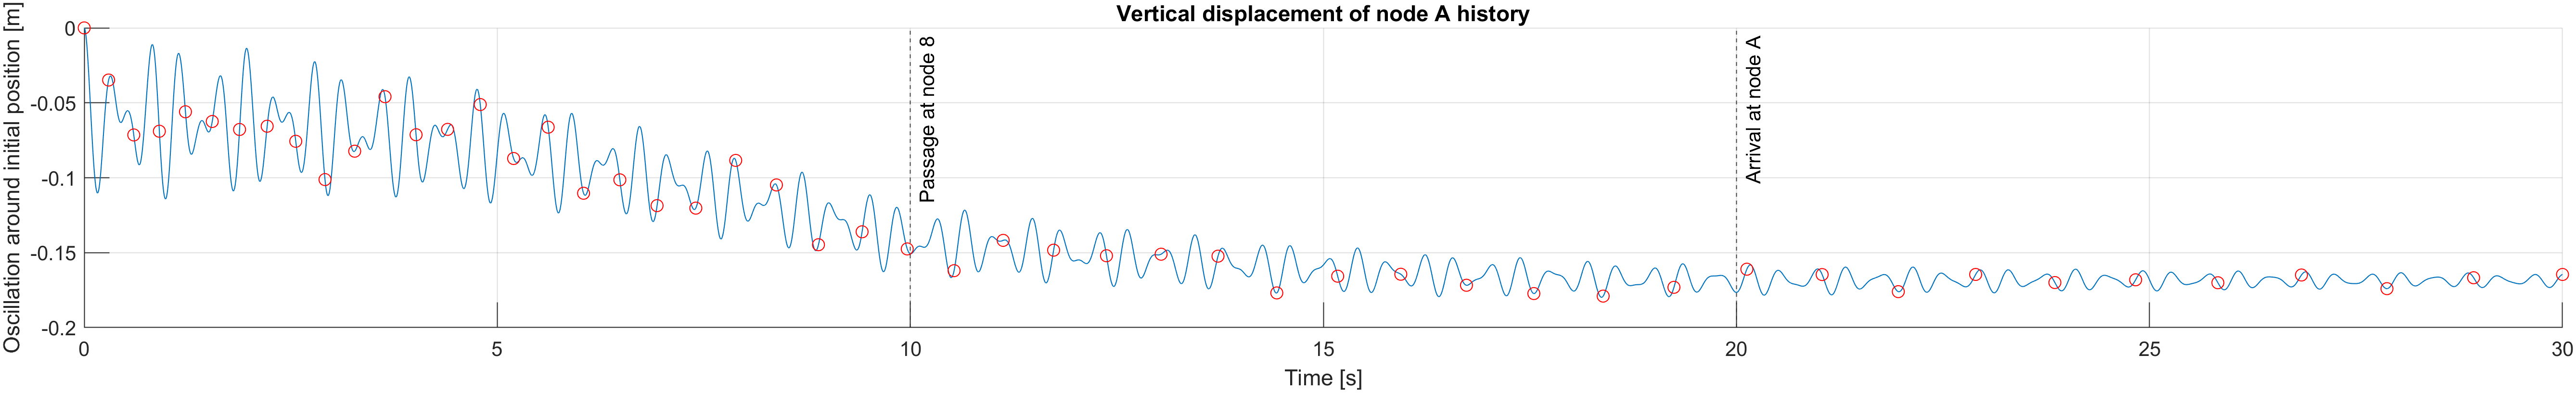
\includegraphics[width=\textwidth]{img/MATLAB/Responses/Moving_load_history_condition_1.png}
    \caption{Dynamic response of the structure due to the moving load (initial condition 1)}
    \label{fig:moving_loads_response_initial_condition_1}
\end{figure}

As we can see from the time history of node A, the structure shows a fast dynamic response due to the sudden addition of the load (in some sense this might be seen as a shock/impact response), over imposed to a slow dynamic response due to the moving load.

\paragraph{Initial condition 2}

In this case, the structure is in its deformed configuration due to the static loads of the mass, which then starts to move along the $x$ axis at $t = 0$.

\begin{figure}[H]
    \centering
    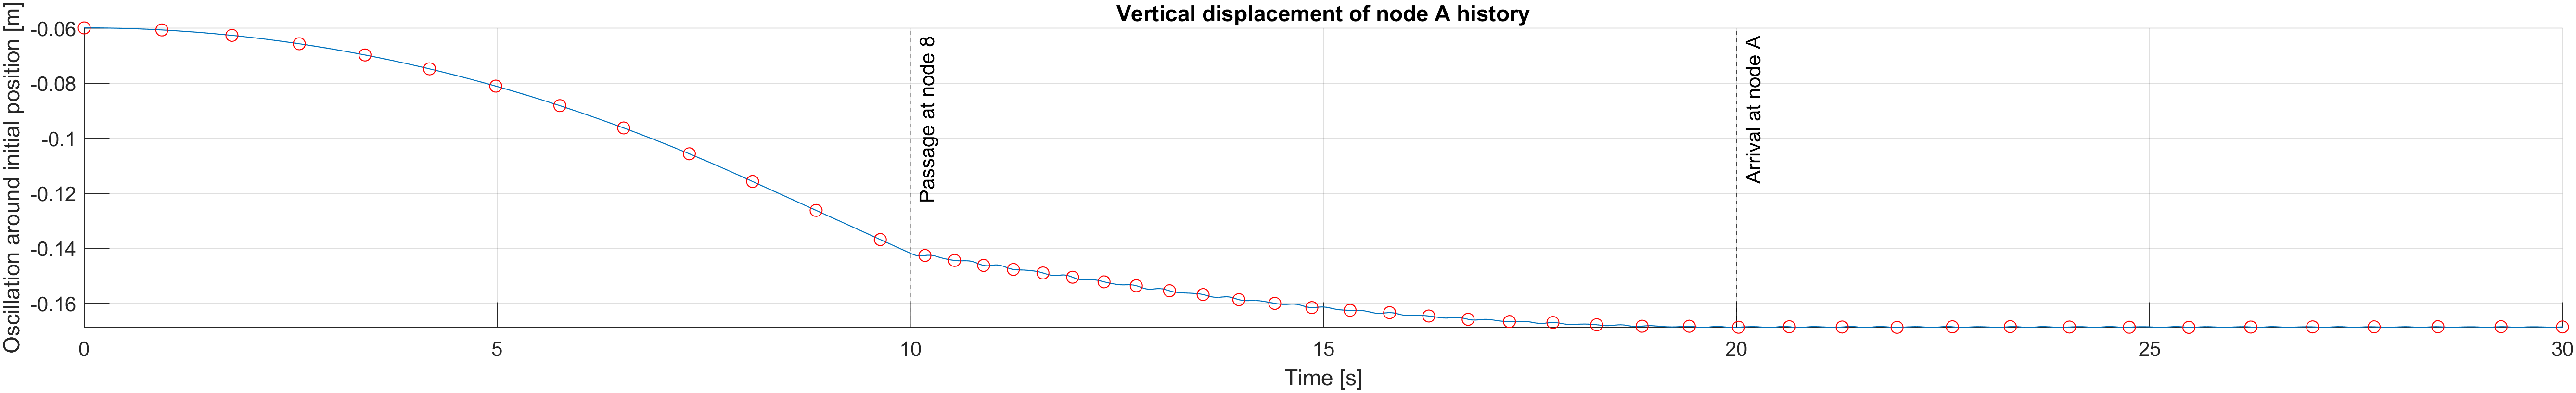
\includegraphics[width=\textwidth]{img/MATLAB/Responses/Moving_load_history_condition_2.png}
    \caption{Dynamic response of the structure due to the moving load (initial condition 2)}
    \label{fig:moving_loads_response_initial_condition_2}
\end{figure}

As we can see from the time history of node A, the structure shows a much more steady and controlled response, with no strong oscillatory behavior.
This can be explained by the absence of the equivalent shock/impact response due to the sudden addition of the load.
